\documentclass{beamer}
 
%presentation pre-amble
\input{./Presentation_MathsPreamble}
%Preamble file for all presentation styles but not including maths formatting!

\usepackage[utf8]{inputenc}

\usepackage{graphicx}
\usepackage{subfigure}
\usepackage{tikz}
\usetikzlibrary{arrows}

\usetheme{Madrid}
\usecolortheme{default}
 
%removes figure prefix from captions
\setbeamertemplate{caption}{\raggedright\insertcaption\par}

%sets the directory for image files - note: this assumes the file structure as of 14-10-2019
\graphicspath{{../Diagrams/Diagram_PDFs/} {../Images/}}

\usepackage{soul} %strikethrough text via \st
\usepackage{graphicx}
\graphicspath{{./PSS_Diagrams/}}
\usepackage{ifthen}

\usepackage{tikz}
\newcommand{\cross}[2]{
\begin{scope}[shift={#1}]
	\filldraw[black!30!white] (-#2,-#2) -- (-#2,-1) -- (#2,-1) -- (#2,-#2) -- (1,-#2) -- (1,#2) -- (#2,#2) -- (#2,1) -- (-#2,1) -- (-#2,#2) -- (-1,#2) -- (-1,-#2) -- cycle;
\end{scope}
}
\newcommand{\eps}{\varepsilon}

%Information to be included in the title page
\title{PDEs on Singular Structures}
\author{William Graham}
\institute{Postgraduate Seminar Series}
\date{\today}
 
\begin{document}
 
\frame{\titlepage}
 
%insert a contents or overview slide at the end
\begin{frame}
	\frametitle{Talk overview}
	
	\begin{enumerate}
		\item Introduction and Motivation
		\item Singular structures and boundary conditions
		\item A New Calculus
		\item The End Product
		\item Conclusion and Summary
	\end{enumerate}
\end{frame}

%Motivation 1
\begin{frame}
	\frametitle{\st{The Part Where I Attempt to Convince You Analysis has Practical Applications} Motivation}
	
	\visible<1->{
	\begin{block}{Modelling using PDEs}
		A physical model for a real-world process typically involves:
		\begin{itemize}
			\item A governing equation
			\item A domain
			\item Boundary data/conditions
		\end{itemize}
	\end{block}
	}%
	
	\visible<2->{
	The governing equation \textit{tends} to vary only with the modelling context:
	\begin{itemize}
		\item Concerning fluids: Naiver-Stokes, Shallow Water, Porous Flow
		\item Concerning electromagnetism: Maxwell, (Modal) Wave Equation
		\item Concerning material warping: Linear elasticity, Naiver-Cauchy
	\end{itemize}
	The boundary conditions reflect physical restrictions on the process.
	}%
	
\end{frame} 

\begin{frame}
	
	\begin{overprint}
	The domain details the physical space the model occupies.
	\end{overprint}
	\begin{columns}
		\begin{column}{0.35\textwidth}
			\begin{overprint}
			Many physical processes require the domain to be separated into regions of differing behaviours.
			\end{overprint}
			\only<1>{
			Layered domain:
			\begin{itemize}
				\item Laminated materials (elasticity)
				\item Non-mixing flows (fluids)
			\end{itemize}
			}
			\only<2>{
			Inclusion domain:
			\begin{itemize}
				\item Cracked materials (elasticity)
				\item Optical fibres (electromagnetism)
			\end{itemize}
			}
			\only<3>{
			Two materials forming a periodic lattice:
			\begin{itemize}
				\item Latticed materials (elasticity)
				\item Photonic crystals (electromagnetism)
			\end{itemize}
			}
		\end{column}
		\begin{column}{0.55\textwidth}
			\only<1>{
			\begin{figure}
				\centering
				\includegraphics[scale=1.0]{LayeredDomain.pdf}
			\end{figure}
			}
			\only<2>{
			\begin{figure}
				\centering
				\includegraphics[scale=1.0]{InclusionDomain.pdf}
			\end{figure}
			}
			\only<3>{
			\begin{figure}
				\centering
				\includegraphics[scale=1.0]{PeriodicCrossDomain.pdf}
			\end{figure}
			}
		\end{column}
	\end{columns}
\end{frame}

%Motivation 3
\begin{frame}
	
	\begin{columns}
		\begin{column}{0.55\textwidth}
				\begin{figure}
					\centering
					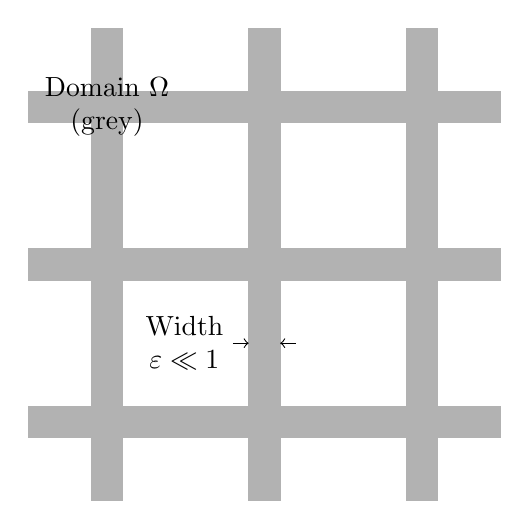
\begin{tikzpicture}
							\foreach \y in {0, ..., 1}
								\foreach \x in {0, ..., 1}
									\cross{(\x*2,\y*2)}{0.2}
									\cross{(-\x*2,-\y*2)}{0.2}
									\cross{(\x*2, -\y*2)}{0.2}
									\cross{(-\x*2,\y*2)}{0.2}
									; %end for \x
								] %end for \y
								
								%domain label
								\node[align=center] at (-2.,2.) {Domain $\Omega$ \\ (grey)};
								%governing equation on domain
								%\node[align=center] at (0,0) {$-\nabla^2 u = \omega^2 u$};
								%boundary conditions
								%\node[align=center] at (1,1) {$\pdiff{u}{\mathbf{n}}\big\vert_{\partial\Omega}=0$};
								%thickness
								\draw[->] (-0.4,-1) -- (-0.2,-1);
								\draw[->] (0.4,-1) -- (0.2,-1);
								\node[align=center, anchor=east] at (-0.4,-1) {Width \\ $\eps\ll 1$};
					\end{tikzpicture}
				\end{figure}
		\end{column}
		\begin{column}{0.35\textwidth}
			\begin{block}{Thin Domains}
				\begin{itemize}
					\item Typically the ``width" of $\ddom$, $\eps\ll 1$.
					\item Computationally solvable, but typically not analytically.
				\end{itemize}
			\end{block}
			\visible<2->{
			\begin{block}{The Plan}
				Can we obtain an analytically solvable \emph{approximate} model?
			\end{block}
			}
		\end{column}
	\end{columns}
\end{frame}

%Singular Structures
\begin{frame}
	\frametitle{Singular-Structures}
	
	In pictures, it looks like
	\begin{figure}
		\centering
		\includegraphics[scale=0.5]{Domain_Illustrations.pdf}
	\end{figure}
	
	The domain on the right is a ``singular structure" - it has \emph{no width}, or \emph{no area}.
	\visible<2->{
	\alert{But what happens to the PDE and the boundary conditions as $\eps\rightarrow0$?}
	}
	
\end{frame}

%Singular Structures: Boundary Conditions
\begin{frame}
	\frametitle{One Problem: Boundary Conditions}
	
	\only<1-2>{
	Suppose we are considering
	\begin{align*}
		-\grad^2 u = \omega^2 u, &\quad
		\pdiff{u}{\mathbf{n}}\big\vert_{\partial\ddom} = 0.
	\end{align*}
	on the domain:
	\begin{figure}
		\centering
		\begin{tikzpicture}
			\filldraw[black!30!white] (-0.2,-1) rectangle (0.2,1);
			\filldraw[black!30!white] (-1,-0.2) rectangle (1,0.2);

			\node[align=center] at (1.5,0) {\large $\overset{\varepsilon\rightarrow 0}{\longrightarrow}$};		
			
			\begin{scope}[shift={(3,0)}]
				\draw[black!30!white] (-1,0) -- (1,0);
				\draw[black!30!white] (0,-1) -- (0,1);
			\end{scope}
		\end{tikzpicture}
	\end{figure}

	\begin{figure}
		\centering
		\begin{subfigure}[t!]{0.45\textwidth}
			\centering
			\includegraphics[scale=1.0]{BoundaryCondition_Diagram.pdf}
			\caption{Non-singular domain: $\frac{\partial u}{\partial \mathbf{n}}$ makes sense.}
		\end{subfigure}
		~
		\visible<2->{
		\begin{subfigure}[t!]{0.45\textwidth}
			\centering
			\includegraphics[scale=1.0]{BoundaryConditionSingularProblem.pdf}
			\caption{Singular domain: $\frac{\partial u}{\partial \mathbf{n}}$ doesn't make sense. }
		\end{subfigure}
		}
	\end{figure}
	}
	
	\only<3>{
	\begin{figure}
		\centering
		\includegraphics[scale=0.35]{BoundaryConditionsDealWith_Drake.jpg}
	\end{figure}
	}
\end{frame}

\begin{frame}	
	\visible<1->{
	Take our problem,
	\begin{align*}
		-\grad^2 u = \omega^2 u, &\quad
		\pdiff{u}{\mathbf{n}}\big\vert_{\partial\ddom} = 0.
	\end{align*}
	}
	\visible<2->{
	Multiply by a test function $\phi\in\smooth{\ddom}$ and integrate,
	\begin{align*}
		-\integral{\ddom}{\phi\grad^2 u}{\mathbf{x}} = \integral{\ddom}{\omega^2 u\phi}{\mathbf{x}}.
	\end{align*}
	}
	\visible<3->{
	Use integration by parts and the boundary condition,
	\begin{align*}
		-\integral{\ddom}{\phi\grad^2 u}{\mathbf{x}} &= \integral{\ddom}{\grad u\cdot\grad\phi}{\mathbf{x}} - \underbrace{\integral{\partial\ddom}{\phi \pdiff{u}{\mathbf{n}}}{s}}_{=0}
	\end{align*}
	}
	\visible<4->{
	Write the weak form:
	\begin{align*}
		\integral{\ddom}{\grad u\cdot\grad\phi - \omega^2 u\phi}{\mathbf{x}} &= 0 \quad\forall \phi\in\smooth{\ddom}
	\end{align*}
	\alert{And pretend we started from there.}
	}
\end{frame}

\begin{frame}
	\frametitle{More problems}
	
	\only<1-2>{
	We have taken care of the boundary conditions, but...	
	\visible<1->{
	\begin{figure}
		\centering
		\includegraphics[scale=0.4]{NeedForMeasureTheory_Gru.jpg}
	\end{figure}
	}
	\visible<2>{
	\alert{So every function $u$ would be a solution to this problem...}
	}
	}
	
	\only<3-4>{
	\begin{block}{How do we fix this?}
		\begin{itemize}
			\item \st{Give up and try to salvage your PhD}
			\item Singular structure having ``no area" is the problem.
			\item If we could somehow change the way we integrate so that our structure didn't have ``zero area" we might be able to move forward.
		\end{itemize}
		\visible<4->{
		\begin{columns}
			\begin{column}{0.45\textwidth}
				Hence, we are going to need to take a small detour and talk about Measure Theory.
			\end{column}
			\begin{column}{0.45\textwidth}
				\begin{figure}
					\centering
					\includegraphics[scale=0.25]{MentionMeasureTheory_Sponguebob.jpg}
				\end{figure}
			\end{column}
		\end{columns}
		}
	\end{block}
	}
\end{frame}

\begin{frame}
	\frametitle{Measure Theory}
	
	\visible<1->{
	\begin{block}{What's a measure?}
		A measure is a function $\nu$ that takes a set $B$ as an input, and returns the ``size" or ``measure" of $B$, $\nu\bracs{B}$.
	\end{block}
	}
	
	\only<1>{
	Lebesgue measure in $\reals^n$: $\lambda_n$.
	\begin{itemize}
		\item $\lambda_1\bracs{\sqbracs{a,b}} = b-a$ (length of a line)
		\item $\lambda_2$ is the usual idea of area
		\item $\lambda_3$ is the usual idea of volume
	\end{itemize}
	}
	\only<2>{
	Point-mass measure $\delta_x$:
	\begin{align*}
		\delta_x\bracs{B} = \begin{cases} 1 & x\in B, \\ 0 & x\not\in B. \end{cases}
	\end{align*}
	``A set has size 1 if it contains the point $x$, otherwise it has no size".
	}
	\only<3>{
	Singular-measures: \newline
	\begin{columns}
		\begin{column}{0.45\textwidth}
			If $I$ is a line segment in $\reals^n$, then
			\begin{align*}
				\lambda_I\bracs{B} &= \lambda_1\bracs{B\cap I}.
			\end{align*}
			If $\ddom = I_1\cup I_2\cup ... I_N$, then use the singular measure
			\begin{align*}
				\ddmes &= \sum_{n=1}^N \lambda_{I_{n}}
			\end{align*}
		\end{column}
		\begin{column}{0.45\textwidth}
			\begin{figure}
				\centering
				\includegraphics[scale=1.0]{SingularMeasureSegment_Diagram.pdf}
			\end{figure}
		\end{column}
	\end{columns}
	}
\end{frame}

\begin{frame}
	\frametitle{Integration}
	
	Integration is still ``area under the curve", only with our new definition of ``area".
	\only<1>{
	\begin{figure}
		\centering
		\includegraphics[scale=0.65]{RiemannIntegration.pdf}
	\end{figure}
	\begin{align*}
		\int_{x_0}^{x_N} f \ \mathrm{d}x = \lim_{N\rightarrow\infty}\sum_{n=1}^N f(x_{n-1})(x_{n}-x_{n-1})
	\end{align*}
	}
	\only<2>{
	\begin{figure}
		\centering
		\includegraphics[scale=0.65]{MeasureTheoryIntegration.pdf}
	\end{figure}
	\begin{align*}
		\int_{\ddom} f \ \mathrm{d}\nu = \lim_{N\rightarrow\infty}\sum_{n=1}^N \bracs{max_{I_n}f - min_{I_n}f}^*\nu(I_n)
	\end{align*}
	}
	\visible<2>{	
	$^*$ Technically more measure theory stuff but we'll ignore this
	}
	
\end{frame}

\begin{frame}
	Some examples:
	\begin{itemize}
		\item Lebesgue measure is ``normal integration":
		\begin{align*}
			\int_{\sqbracs{a,b}} f(x) \ \md \lambda_1 &= \int_a^b f(x) \md x, \\
			\int_{S} f(x) \ \md \lambda_2 &= \text{Surface integral of } f \text{ over } S, \\
			\int_{\ddom} f(x) \ \md \lambda_3 &= \text{Volume integral of } f \text{ over } \ddom.
		\end{align*}
		\item Point-mass measure is ``Delta-integral":
		\begin{align*}
			\int_{\sqbracs{a,b}} f \ \md \delta_x &= \int_a^b f(t)\delta\bracs{t-x} \ \md t
			= \begin{cases} f(x) & x\in\sqbracs{a,b}, \\ 0 & x\not\in\sqbracs{a,b}. \end{cases}
		\end{align*}
	\end{itemize}
\end{frame}

\begin{frame}
	\frametitle{Gradients}
	Square-integrable functions live in $\ltwo{\ddom}{\nu} = \clbracs{f \ \vert \ \int_{\ddom}f^2 \ \md\nu < \infty}$. \newline
	
	Having reworked integration, we also need to rework gradients/derivatives.
	\begin{block}{Gradients (technical)}
		$u\in\ltwo{\ddom}{\nu}$ has $\nu$-gradient $z$ if $\exists \varphi_n\in\smooth{\ddom}$ s.t.
		\begin{align*}
			\integral{\ddom}{\varphi_n^2}{\nu} &\rightarrow \integral{\ddom}{u^2}{\nu}, &\quad (\varphi\approx u) \\
			 \integral{\ddom}{\abs{\grad\varphi_n}^2}{\nu} &\rightarrow \integral{\ddom}{\abs{z}^2}{\nu}. &\quad (\grad\varphi\approx z)
		\end{align*}
		$\toInfty{n}$ (convergences in $\ltwo{\ddom}{\nu}$).
	\end{block}
	\alert{``If $\varphi_n$ gets close to $u$, the gradients get close to the gradient of $u$".}
\end{frame}

\begin{frame}
	Alas, there is another problem we run into... \newline
	
	Suppose 
	\begin{align*}
		\varphi\approx u, &\quad \grad\varphi\approx z_1, \\
		\psi\approx 0, &\quad \grad\psi\approx z_2, \\
		\visible<2->{
		\implies \varphi+\psi\approx u, &\quad \grad\bracs{\varphi+\psi}\approx z_1+z_2.
		}
	\end{align*}
	\visible<3->{
	So... $u$ doesn't have only one gradient. \newline
	}
	\visible<4->{
	It actually has infinitely many...
	}
	\visible<5->{
	Oops?
	}
	
\end{frame}

\begin{frame}
	\frametitle{Recap}
	
	\begin{columns}
		\begin{column}{0.45\textwidth}
			So far, we have:
			\begin{block}{Reworked integration}
				\begin{itemize}
					\item Good luck actually doing an integral now
					\item No integration by parts
					\item Still have substitution though!
				\end{itemize}
			\end{block}
			\visible<2->{
			\begin{block}{Reworked derivatives}
				\begin{itemize}
					\item Gradients are found by approximating functions
					\item Every function has infinitely many gradients
					\item No chain- or product rule
				\end{itemize}								
			\end{block}						
			}
		\end{column}
		\begin{column}{0.45\textwidth}
			\visible<3->{
			\begin{figure}
				\centering
				\includegraphics[scale=0.4]{ThisIsFine.jpg}
				\caption{Me $\approx$ 6 months into this PhD}
			\end{figure}
			}
		\end{column}
	\end{columns}
\end{frame}

\begin{frame}
	\frametitle{The Fix}
	
	\begin{block}{Gradients of Zero}
		If $\psi\approx 0, \grad\psi\approx z$ we call $z$ a \emph{Gradient of Zero}. \newline
		$\gradZero{\ddom}{\nu} = \clbracs{z \ \vert \ \psi\approx 0, \grad\psi\approx z}$ is the set of all gradients of zero.
	\end{block}		
	Every function $u$ has \emph{a unique} gradient $\grad_{\nu}u$ such that
	\begin{align*}
		\integral{\ddom}{\grad_\nu u \cdot z}{\nu} &= 0 \quad \forall z\in\gradZero{\ddom}{\nu}.
	\end{align*}
	\begin{block}{Gradients of zero are directions that our measure cannot see}
		$\grad_{\nu}u$ holds all the information we need, all the other gradients of $u$ don't add anything. \newline
		$\grad_{\nu}u$ is the \emph{tangential gradient} of $u$.
	\end{block}
	
\end{frame}

\begin{frame}
	\frametitle{So for Singular Structures...}
	
	\begin{columns}
		\begin{column}{0.45\textwidth}
			If $I$ is a line segment in $\reals^n$, then
			\begin{align*}
				\lambda_I\bracs{B} &= \lambda_1\bracs{B\cap I}.
			\end{align*}
			\visible<2->{
			Tangential gradients correspond to ``gradients in the direction of $I$". \newline
			}
			
			\visible<3>{
			A singular structure with lots of segments gives this behaviour on each segment.
			}
		\end{column}
		\begin{column}{0.45\textwidth}
			\begin{figure}
				\centering
				\only<1>{
				\includegraphics[scale=1.0]{SingularMeasureSegment_Diagram.pdf}
				}
				\only<2->{
				\includegraphics[scale=1.0]{Diagram_GradZero.pdf}
				}
			\end{figure}
		\end{column}
	\end{columns}
\end{frame}

\begin{frame}
	\frametitle{So what do we have?}
	
	Our original problem:
	\begin{columns}
		\begin{column}{0.35\textwidth}
			\begin{align*}
				-\grad^2 u = \omega^2 u 
				&\quad \pdiff{u}{\mathbf{n}}\big\vert_{\partial\ddom} = 0.
			\end{align*}
		\end{column}
		\begin{column}{0.45\textwidth}
			\begin{figure}
				\centering
				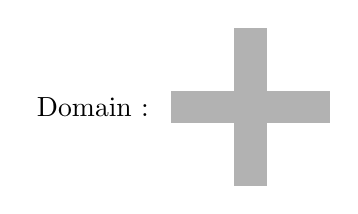
\begin{tikzpicture}
					\node[align=center] at (-2,0) {Domain $\ddom$:};
					\filldraw[black!30!white] (-0.2,-1) rectangle (0.2,1);
					\filldraw[black!30!white] (-1,-0.2) rectangle (1,0.2);
				\end{tikzpicture}
			\end{figure}
		\end{column}
	\end{columns}
	\visible<2->{
	Is approximated by the problem of finding $u\in\ltwo{\ddom}{\ddmes}$ such that
	\begin{align*}
		\integral{\ddom}{\grad_{\ddmes}u\cdot\grad_{\ddmes}\phi - \omega^2u\phi}{\ddmes} &=0, \quad \forall \phi\in\smooth{\ddom},
	\end{align*}
	\begin{columns}
		\begin{column}{0.35\textwidth}
			(where $\ddmes = \sum_{n=1}^4 \lambda_{I_n}$).
		\end{column}
		\begin{column}{0.45\textwidth}
			\begin{figure}
				\centering
				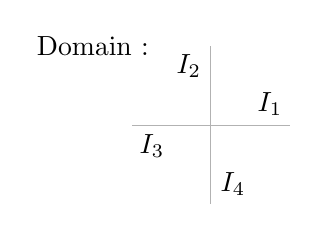
\begin{tikzpicture}
					\node[align=center] at (-1.5,1) {Domain $\ddom$:};
					\draw[black!30!white] (-1,0) -- (1,0);
					\draw[black!30!white] (0,-1) -- (0,1);
					\node[anchor=south] at (0.75,0) {$I_1$};
					\node[anchor=east] at (0,0.75) {$I_2$};
					\node[anchor=north] at (-0.75,0) {$I_3$};
					\node[anchor=west] at (0,-0.75) {$I_4$};
				\end{tikzpicture}
			\end{figure}
		\end{column}
	\end{columns}
	}
\end{frame}

\begin{frame}
	\frametitle{And this is better how?}
	
	\begin{overprint}
	\begin{figure}
		\centering
		\begin{tikzpicture}
			\only<1-2>{
			\node[align=center] at (0,0) {\Large $\integral{\ddom}{\grad_{\ddmes}u\cdot\grad_{\ddmes}\phi - \omega^2u\phi}{\ddmes} =0$};
			}
			\only<2>{
			\draw[thick, red] (1.85,0) circle (.35);
			}
			
			\only<3>{
			\node[align=center] at (0,0) {\Large $\integral{I}{\grad_{\lambda_I}u\cdot\grad_{\lambda_I}\phi - \omega^2u\phi}{\lambda_I} =0$};
			\draw[thick, red] (-2.15,0) circle (.55);
			}
			
			\only<4-5>{
			\node[align=center] at (0,0) {\Large $\integral{I}{\grad_{\lambda_I}u\cdot\grad_{\lambda_I}\phi - \omega^2u\phi}{\lambda_I} =0$};
			}
			\only<4>{
			\draw[thick, red] (2,0) circle (.4);			
			}
		\end{tikzpicture}	
	\end{figure}
	The problem: Find $u\in\ltwo{\ddom}{\mu}$ such that
	\end{overprint}
	
	\only<1>{
	\begin{align*}
		\integral{\ddom}{\grad_{\ddmes}u\cdot\grad_{\ddmes}\phi - \omega^2u\phi}{\ddmes} &=0, \quad \forall \phi\in\smooth{\ddom},
	\end{align*}
	}
	\only<2>{
	\begin{align*}
		\integral{I}{\grad_{\lambda_I}u\cdot\grad_{\lambda_I}\phi - \omega^2u\phi}{\lambda_I} =0, &\quad \forall \phi\in\smooth{\ddom}, \ \forall I\subset\ddom, \\
		u\vert_{I_{j}} = u\vert_{I_{k}}, &\quad \text{where } I_j \cap I_k \neq \emptyset.
	\end{align*}
	Properties of this measure allow us to look at an equation on each line segment, linked at the ``joins".
	}
	\only<3>{
	\begin{align*}
		\integral{I}{ u' \cdot \phi' - \omega^2u\phi}{\lambda_I} =0, &\quad \forall \phi\in\smooth{\ddom}, \ \forall I\subset\ddom, \\
		u\vert_{I_{j}} = u\vert_{I_{k}}, &\quad \text{where } I_j \cap I_k \neq \emptyset.
	\end{align*}
	On each edge, $\grad_{\ddmes}u$ can be written as a function of one variable, along the line segment $I$.
	}
	\only<4>{
	\begin{align*}
		\int_{0}^{\abs{I}} \tilde{u}' \cdot \tilde{\phi}' - \omega^2 \tilde{u}\tilde{\phi} \ \md t =0, &\quad \forall \tilde{\phi}\in\smooth{\interval{I}}, \ \forall I\subset\ddom, \\
		u\vert_{I_{j}} = u\vert_{I_{k}}, &\quad \text{where } I_j \cap I_k \neq \emptyset.
	\end{align*}
	Using integration by substitution, we can transform this into a \emph{normal} Lebesgue integral, with familiar derivatives $\tilde{u}'$.
	}
	\only<5>{
	\begin{align*}
		-\tilde{u}''(t) = \omega^2 \tilde{u}(t), \ t\in\interval{I}, &\quad \forall I\subset\ddom, \\
		u\vert_{I_{j}} = u\vert_{I_{k}}, &\quad \text{where } I_j \cap I_k \neq \emptyset, \\
		\sum_{\text{Junctions}}u' = 0, &\quad\text{(Kirchoff condition, annoying notation)}.
	\end{align*}
	As this is normal Lebesgue integration, we can go from the weak form to the strong form, \alert{and we have a system of ODEs!}
	}
\end{frame}

\begin{frame}
	\frametitle{Summary}
	
	Originally:
	\begin{columns}
		\begin{column}{0.45\textwidth}
			\begin{figure}
				\centering
				
\begin{tikzpicture}
					\filldraw[black!30!white] (-0.2,-1) rectangle (0.2,1);
					\filldraw[black!30!white] (-1,-0.2) rectangle (1,0.2);
				\end{tikzpicture}
			\end{figure}
		\end{column}
		\begin{column}{0.45\textwidth}
			\begin{align*}
				-\grad^2 u = \omega^2 u, &\quad
				\pdiff{u}{\mathbf{n}}\big\vert_{\partial\ddom} = 0.
			\end{align*}
			PDE to solve on thin domains, hard to solve analytically.
		\end{column}
	\end{columns}
	
	\vspace{2mm}
	
	Now approximated by:
	\begin{columns}
		\begin{column}{0.45\textwidth}
			\begin{itemize}
				\item One ODE per segment
				\item Matching conditions at the ``connections"
				\item Easily solvable computationally
				\item Solvable analytically
			\end{itemize}
		\end{column}
		\begin{column}{0.45\textwidth}
			\begin{figure}
				\centering
				\begin{tikzpicture}
					\draw[black!30!white] (-1,0) -- (1,0);
					\draw[black!30!white] (0,-1) -- (0,1);
					\node[anchor=south] at (0.75,0) {$I_1$};
					\node[anchor=east] at (0,0.75) {$I_2$};
					\node[anchor=north] at (-0.75,0) {$I_3$};
					\node[anchor=west] at (0,-0.75) {$I_4$};
				\end{tikzpicture}
			\end{figure}
		\end{column}
	\end{columns}
\end{frame}

\begin{frame}
	\frametitle{\st{Check if anyone has made it to the end} Conclusion}
	
	\begin{block}{Approximate PDEs on thin domains by ODEs on singular domains}
		\begin{itemize}
			\visible<2->{
			\item Write problem in weak form
			}
			\visible<3->{
			\item Change the definition of area that we are using
			}
			\visible<4->{
			\item Rework derivatives
			}
			\visible<5->{
			\item Put out all the fires that this caused
			}
			\visible<6->{
			\item Obtain an approximation, that can be tackled analytically
			}
		\end{itemize}
	\end{block}
	
	\begin{block}{This is good because?}
		\begin{itemize}
			\visible<7->{
			\item ODEs are easier to deal with than PDEs (analytically and computationally)
			}
			\visible<8->{
			\item The hard work (reworking integration, differentiation) only needs be done once
			}
			\visible<9->{
			\item (It gets me a PhD)
			}
		\end{itemize}
	\end{block}

\end{frame}

\begin{frame}
	
	\begin{block}{Thank you for sticking through to the end}
		\centering
		Any questions?
		Or regrets from listening?
	\end{block}
\end{frame}

\end{document}
